
\documentclass[12pt]{standalone}
\usepackage{tikz}
\usetikzlibrary{automata,positioning}
\begin{document}
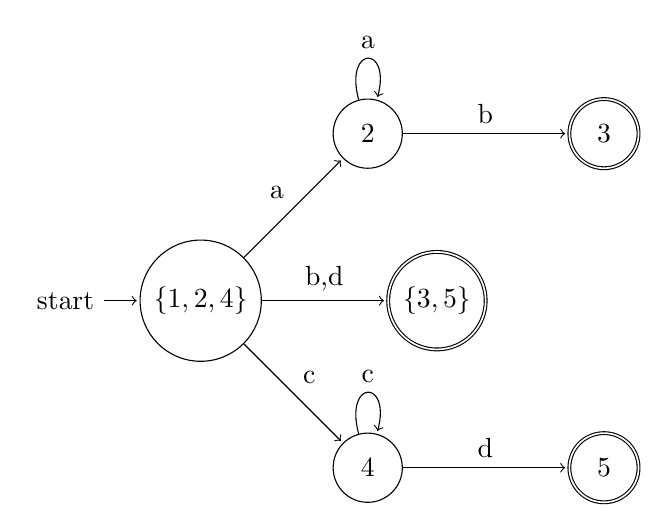
\begin{tikzpicture}[shorten >=1pt,node distance=3cm,on grid,auto] 
   \node[state, initial] (0) {$\{1,2,4\}$}; 
   \node[state] (1) [above right=of 0] {$2$};
   \node[state] (2) [below right=of 0] {$4$};
    \node[state, accepting] (3) [right=of 1] {$3$};
    \node[state, accepting] (4) [right=of 2] {$5$};
    \node[state, accepting] (5) [right=of 0] {$\{3,5\}$};

    \path[->] (0) edge  node {a} (1);
    \path[->] (0) edge  node {c} (2);
    \path[->] (0) edge  node {b,d} (5);
    
    \path[->] (1) edge [loop above] node  {a} (1);
    \path[->] (1) edge node {b} (3);
    
    \path[->] (2) edge [loop above] node  {c} (2);
    \path[->] (2) edge  node {d} (4);
\end{tikzpicture}
\end{document}  

